% arara: pdflatex: { shell: on }
% arara: biber
% arara: pdflatex: { shell: on }
% arara: pdflatex: { shell: on }
% arara: biber
% arara: pdflatex: { shell: on }
%% arara: clean: { files: [ Masterarbeit_Grieco_1408410.aux, Masterarbeit_Grieco_1408410.bbl, Masterarbeit_Grieco_1408410.bcf, Masterarbeit_Grieco_1408410.cod, Masterarbeit_Grieco_1408410.blg, Masterarbeit_Grieco_1408410.lof, Masterarbeit_Grieco_1408410.lot, Masterarbeit_Grieco_1408410.out, Masterarbeit_Grieco_1408410.toc, Masterarbeit_Grieco_1408410.log, Masterarbeit_Grieco_1408410.lol, Masterarbeit_Grieco_1408410.run.xml, _minted-Masterarbeit_Grieco_1408410 ] } 

\documentclass[
    12pt, % Schriftgröße
    DIV10,
    ngerman, % für Umlaute, Silbentrennung etc.
    a4paper, % Papierformat
    oneside, % einseitiges Dokument
    titlepage, % es wird eine Titelseite verwendet
    parskip=half, % Abstand zwischen Absätzen (halbe Zeile)
    headings=normal, % Größe der Überschriften verkleinern
    listof=totoc, % Verzeichnisse im Inhaltsverzeichnis aufführen
    bibliography=totoc, % Literaturverzeichnis im Inhaltsverzeichnis aufführen
    index=totoc, % Index im Inhaltsverzeichnis aufführen
    captions=tableheading, % Beschriftung von Tabellen unterhalb ausgeben
    final % Status des Dokuments (final/draft)
]{scrreprt}

% Weise compiler an, nicht bei Fehlern anzuhalten!
%\nonstopmode

% benötigte Packages -----------------------------------------------------------
%   LaTeX-Packages, die benötigt werden, sind in die Datei Packages.tex
%   "ausgelagert", um diese Vorlage möglichst übersichtlich zu halten.
% ------------------------------------------------------------------------------
% Anpassung des Seitenlayouts --------------------------------------------------
%   siehe Seitenstil.tex
% ------------------------------------------------------------------------------
\usepackage[
    automark, % Kapitelangaben in Kopfzeile automatisch erstellen
    headsepline, % Trennlinie unter Kopfzeile
    ilines % Trennlinie linksbündig ausrichten
]{scrlayer-scrpage}

% Anpassung an Landessprache ---------------------------------------------------
\usepackage[ngerman,showlanguages]{babel}

% Umlaute ----------------------------------------------------------------------
%   Umlaute/Sonderzeichen wie äüöß direkt im Quelltext verwenden (CodePage).
%   Erlaubt automatische Trennung von Worten mit Umlauten.
% ------------------------------------------------------------------------------
\usepackage[utf8]{inputenc}
\usepackage[T1]{fontenc}
\usepackage{textcomp} % Euro-Zeichen etc.

% Schrift ----------------------------------------------------------------------
\usepackage{lmodern} % bessere Fonts
\usepackage{relsize} % Schriftgröße relativ festlegen

% Grafiken ---------------------------------------------------------------------
% Einbinden von JPG-Grafiken ermöglichen
%\usepackage[dvips,final]{graphicx}
% hier liegen die Bilder des Dokuments
%\graphicspath{{Bilder/}}

% Befehle aus AMSTeX für mathematische Symbole z.B. \boldsymbol \mathbb --------
\usepackage{amsmath,amsfonts}

% für Index-Ausgabe mit \printindex --------------------------------------------
\usepackage{makeidx}
\makeindex
\AtBeginDocument{\renewcommand\indexname{Stichwortverzeichnis}}
%\addcontentsline{toc}{chapter}{Stichwortverzeichnis}

% Einfache Definition der Zeilenabstände und Seitenränder etc. -----------------
\usepackage{setspace}
\usepackage{geometry}

% Symbolverzeichnis ------------------------------------------------------------
%   Symbolverzeichnisse bequem erstellen. Beruht auf MakeIndex:
%     makeindex.exe %Name%.nlo -s nomencl.ist -o %Name%.nls
%   erzeugt dann das Verzeichnis. Dieser Befehl kann z.B. im TeXnicCenter
%   als Postprozessor eingetragen werden, damit er nicht ständig manuell
%   ausgeführt werden muss.
%   Die Definitionen sind ausgegliedert in die Datei "Glossar.tex".
% ------------------------------------------------------------------------------
% \usepackage[intoc]{nomencl}
% \let\abbrev\nomenclature
% \renewcommand{\nomname}{Abkürzungsverzeichnis}
% \setlength{\nomlabelwidth}{.25\hsize}
% \renewcommand{\nomlabel}[1]{#1 \dotfill}
% \setlength{\nomitemsep}{-\parsep}

% Abkürzungsverzeichnis
\usepackage[printonlyused]{acronym} %Abkürzungsverzeichnis erstellen, Langtext als Fußnote, Auflistung nur bei Verwendung

% zum Umfließen von Bildern ----------------------------------------------------
\usepackage{floatflt}
\usepackage{float}

% Abstand der float caption
\usepackage{caption}
\captionsetup{belowskip=10pt,aboveskip=10pt}

% ensure floats do not go into the next section.
\usepackage[section]{placeins}

% Farben
\usepackage[dvipsnames]{xcolor}
\definecolor{hellgrau}{rgb}{0.93,0.93,0.93}
\definecolor{colKeys}{rgb}{0,0,0.9}
\definecolor{colIdentifier}{rgb}{0,0,0}
\definecolor{colComments}{rgb}{0.6,0,0}
\definecolor{colString}{rgb}{0,0.7,0}

% Farben für Java Diagram
\definecolor{javaProgramm}  {rgb}{0.95, 0.9,    0.5}
\definecolor{javaPackage}   {rgb}{0,    0.7,    0}
\definecolor{javaClass}     {rgb}{0,    0.7,    0.7}
\definecolor{javaAnonClass} {rgb}{0.1,  0.7,    0.7}
\definecolor{javaMethod}    {rgb}{0.7,  0,      0}
\definecolor{javaStatement} {rgb}{1,    0.5,    0}

% zum Einbinden von Programmcode -----------------------------------------------
\usepackage{listings}
\usepackage[newfloat]{minted}

\setminted{
    xleftmargin=20pt,
    linenos=true,
    breaklines
}

\lstset{
    float=hbp,
    basicstyle=\ttfamily\color{black}\small\smaller,
    keywordstyle=\color{colKeys},
    stringstyle=\color{colString},
    commentstyle=\color{colComments},
    columns=flexible,
    tabsize=4,
    frame=single,
    extendedchars=true,
    showspaces=false,
    showstringspaces=false,
    numbers=left,
    numberstyle=\tiny,
    breaklines=true,
    backgroundcolor=\color{hellgrau},
    captionpos=b,
    breakautoindent=true
}

% URL verlinken, lange URLs umbrechen etc. -------------------------------------
\usepackage{url}
\makeatletter
\g@addto@macro{\UrlBreaks}{\UrlOrds}
\makeatother

%% Roman pagenumbers good aligned in toc
%\usepackage{tocloft}
%\cftsetpnumwidth{2em}
%\setlength\cftafterfigskip{10pt}
%\renewcommand\cftchapafterpnum{\vskip10pt}
%\renewcommand\cftsecafterpnum{\vskip15pt}

% fortlaufendes Durchnummerieren der Fußnoten ----------------------------------
\usepackage{chngcntr}

% für lange Tabellen -----------------------------------------------------------
\usepackage{longtable}
\usepackage{array}
\usepackage{ragged2e}

% seiten rotieren
\usepackage{pdflscape}

% Spaltendefinition rechtsbündig mit definierter Breite ------------------------
\newcolumntype{w}[1]{>{\raggedleft\hspace{0pt}}p{#1}}

% Formatierung von Listen ändern -----------------------------------------------
\usepackage{paralist}

% bei der Definition eigener Befehle benötigt
\usepackage{ifthen}

% definiert u.a. die Befehle \todo und \listoftodos
\usepackage{todonotes}

% sorgt dafür, dass Leerzeichen hinter parameterlosen Makros nicht als Makroendezeichen interpretiert werden
\usepackage{xspace}

% einbinden anderer PDF Dateien (Deckblatt etc.)
\usepackage{pdfpages}

% Bibliographics
% Naturwissenschaftliche Bibliographien
%\usepackage[square, comma, numbers]{natbib}
% Stil der Zitate und der Bibliographie
%\bibliographystyle{natdin}
\usepackage[backend=biber]{biblatex}
\addbibresource{Sonstiges/Literatur.bib}

% Tikz libraries
\usepackage{tikz}
\usetikzlibrary{patterns}
\usepackage{tikz-uml}

% Spalten
\usepackage{multicol}

% Anhang
\usepackage[toc,page]{appendix}

% SVG Biler
\usepackage{svg}

% euro sign
\usepackage{eurosym}

% subfigures
\usepackage{subfig}
\usepackage{floatflt}
\usepackage{wrapfig}

% Quotes in babel language
\usepackage{csquotes}


% PDF-Optionen -----------------------------------------------------------------
\usepackage[
    bookmarks,
    bookmarksopen=true,
    colorlinks=true,
% diese Farbdefinitionen zeichnen Links im PDF farblich aus
    linkcolor=black, % einfache interne Verknüpfungen
    anchorcolor=black,% Ankertext
    citecolor=black, % Verweise auf Literaturverzeichniseinträge im Text
    filecolor=black, % Verknüpfungen, die lokale Dateien öffnen
    menucolor=black, % Acrobat-Menüpunkte
    urlcolor=black, 
% diese Farbdefinitionen sollten für den Druck verwendet werden (alles schwarz)
    %linkcolor=black, % einfache interne Verknüpfungen
    %anchorcolor=black, % Ankertext
    %citecolor=black, % Verweise auf Literaturverzeichniseinträge im Text
    %filecolor=black, % Verknüpfungen, die lokale Dateien öffnen
    %menucolor=black, % Acrobat-Menüpunkte
    %urlcolor=black,
    plainpages=false, % zur korrekten Erstellung der Bookmarks
    pdfpagelabels, % zur korrekten Erstellung der Bookmarks
    hypertexnames=true, % zur korrekten Erstellung der Bookmarks
    linktoc=all, % Seitenzahlen und Text im Inhaltsverzeichnis verlinken
]{hyperref}

% Befehle, die Umlaute ausgeben, führen zu Fehlern, wenn sie hyperref als Optionen übergeben werden
\hypersetup{
    pdftitle={\mytitel},
    pdfauthor={\myautor},
    pdfcreator={\myautor},
    pdfsubject={\mytitel},
    pdfkeywords={\mytitel \myart \myautor}
}

% Meta-Informationen -----------------------------------------------------------
%   Informationen über das Dokument, wie z.B. Titel, Autor, Matrikelnr. etc
%   werden in der Datei Meta.tex definiert und können danach global
%   verwendet werden.
% ------------------------------------------------------------------------------
% Meta-Informationen -----------------------------------------------------------
%   Definition von globalen Parametern, die im gesamten Dokument verwendet
%   werden k�nnen (z.B auf dem Deckblatt etc.).
%
%   ACHTUNG: Wenn die Texte Umlaute oder ein Esszet enthalten, muss der folgende
%            Befehl bereits an dieser Stelle aktiviert werden:
%            \usepackage[latin1]{inputenc}
% ------------------------------------------------------------------------------

\newcommand{\mytitel}{Programmiersprachliche Konzepte von COBOL im Vergleich mit Java -- Eine praxisorientierte Einf�hrung}
\newcommand{\myart}{Masterarbeit}
\newcommand{\myfachgebiet}{Informatik und Multimedia}
\newcommand{\myautor}{Antonio Grieco}
\newcommand{\mymatrikelnr}{}
\newcommand{\myerstgutachter}{}
\newcommand{\myzweitgutachter}{}
\newcommand{\myjahr}{2018}
\newcommand{\myort}{Augsburg}

% Kopf- und Fußzeilen, Seitenränder etc. ---------------------------------------
% Zeilenabstand 1,5 Zeilen -----------------------------------------------------
\onehalfspacing

% Seitenränder -----------------------------------------------------------------
\setlength{\topskip}{\ht\strutbox} % behebt Warnung von geometry
\geometry{paper=a4paper,left=30mm,right=25mm,top=25mm,bottom=20mm,footskip=12mm}

% Kopf- und Fußzeilen ----------------------------------------------------------
\pagestyle{scrheadings}
% Kopf- und Fußzeile auch auf Kapitelanfangsseiten
\renewcommand*{\chapterpagestyle}{scrheadings} 
% Schriftform der Kopfzeile
\renewcommand{\headfont}{\normalfont}

% Kopfzeile
% \ihead{\large{\textsc{\titel}}\\ \small{\untertitel}}
\ihead{}
\chead{}
\ohead{\textit{\headmark}}
\setlength{\headheight}{1.1\baselineskip}
%\setlength{\headheight}{21mm} % Höhe der Kopfzeile
% \setheadwidth[0pt]{textwithmarginpar} % Kopfzeile über den Text hinaus verbreitern
\setheadsepline[text]{0.4pt} % Trennlinie unter Kopfzeile
% \setfootsepline[text]{0.4pt} % Trennlinie über Fußzeile

% Fußzeile
\ifoot{}
\cfoot{\pagemark}
\ofoot{}

% sonstige typographische Einstellungen ----------------------------------------

% erzeugt ein wenig mehr Platz hinter einem Punkt
\frenchspacing 

% Schusterjungen und Hurenkinder vermeiden
\clubpenalty = 10000
\widowpenalty = 10000 
\displaywidowpenalty = 10000

% Quellcode-Ausgabe formatieren
\lstset{numbers=left, numberstyle=\tiny, numbersep=5pt, breaklines=true}
\lstset{emph={square}, emphstyle=\color{red}, emph={[2]root,base}, emphstyle={[2]\color{blue}}}

% Fußnoten fortlaufend durchnummerieren
\counterwithout{footnote}{chapter}


% eigene Definitionen für Silbentrennung
% Trennvorschl�ge im Text werden mit \" angegeben
% untrennbare W�rter und Ausnahmen von der normalen Trennung k�nnen in dieser
% Datei mittels \hyphenation definiert werden

% eigene LaTeX-Befehle
% Eigene Befehle und typographische Auszeichnungen für diese

% einfaches Wechseln der Schrift, \zB: \changefont{cmss}{sbc}{n}
\newcommand{\changefont}[3]{\fontfamily{#1} \fontseries{#2} \fontshape{#3} \selectfont}

% Abkürzungen mit korrektem Leerraum 
\newcommand{\bzw}{bzw.\ }
\newcommand{\dahe}{\mbox{d.\,h.\ }}
\newcommand{\engl}{engl.\ }
\newcommand{\evtl}{evtl.\ }
\newcommand{\ggf}{ggf.\ }
\newcommand{\iA}{\mbox{i.\,A.\ }}
\newcommand{\idR}{\mbox{i.\,d.\,R.\ }}
\newcommand{\lat}{lat.\ }
\newcommand{\sog}{sog.\ }
\newcommand{\szs}{szs.\ }
\newcommand{\ua}{\mbox{u.\,a.\ }}
\newcommand{\uA}{\mbox{u.\,A.\ }}
\newcommand{\uU}{\mbox{u.\,U.\ }}
\newcommand{\Vgl}{Vgl.\ }
\newcommand{\zB}{\mbox{z.\,B.\ }}

\newcommand{\abbildung}[1]{Abbildung~\ref{fig:#1}}

\newcommand{\bs}{$\backslash$}

% erzeugt ein Listenelement mit fetter Überschrift 
\newcommand{\itemd}[2]{\item{\textbf{#1}}\\{#2}}

% einige Befehle zum Zitieren --------------------------------------------------
%\newcommand{\Zitat}[2][\empty]{\ifthenelse{\equal{#1}{\empty}}{\citep{#2}}{\citep[#1]{#2}}}

% zum Ausgeben von Autoren
%\newcommand{\AutorName}[1]{\textsc{#1}}
%\newcommand{\Autor}[1]{\AutorName{\citeauthor{#1}}}

% verschiedene Befehle um Wörter semantisch auszuzeichnen ----------------------
\newcommand{\NeuerBegriff}[1]{\textbf{#1}}
\newcommand{\Fachbegriff}[1]{\textit{#1}}

\newcommand{\Eingabe}[1]{\texttt{#1}}
\newcommand{\Code}[1]{\texttt{#1}}
\newcommand{\Datei}[1]{\texttt{#1}}

\newcommand{\Datentyp}[1]{\textsf{#1}}
\newcommand{\XMLElement}[1]{\textsf{#1}}
\newcommand{\Webservice}[1]{\textsf{#1}}

\newcommand{\quotes}[1]{»#1«}

\newcommand{\citeWithTitle}[1]{\citetitle{#1} \cite{#1}}
\newcommand{\citeVgl}[1]{\cite[vgl.][]{#1}}

\newcommand{\till}[2]{#1 -- #2}

%Minted
\usepackage{xparse}
\NewDocumentEnvironment{codeWithCaption}{mm} % one m per argument
  {}
  {
    \vspace*{-3.5em}
    \begingroup\captionsetup{type=listing}\captionof{listing}{#1\label{#2}}\endgroup
  }

\newcommand{\cob}[1]{\mintinline[breaklines]{cobolfree}{#1}}
\newcommand{\jav}[1]{\mintinline[breaklines]{java}{#1}}

\newcommand{\inputCode}[3]{
    \inputminted[frame=lines,framesep=2mm,baselinestretch=1.2,linenos,
    bgcolor=hellgrau,fontsize=#1]{#2}{Code/#3}
}
\newcommand{\cobolNotFree}[1]{\inputCode{\scriptsize}{cobol}{#1}}
\newcommand{\cobol}[1]{\inputCode{\scriptsize}{cobolfree}{#1}}
\newcommand{\java}[1]{\inputCode{\footnotesize}{java}{#1}}

\newcommand{\mintedCobol}[3]{
    \begin{codeWithCaption}{#2}{#3}
    \cobol{#1}
    \end{codeWithCaption}
}

\newcommand{\mintedJava}[3]{
    \begin{codeWithCaption}{#2}{#3}
    \java{#1}
    \end{codeWithCaption}
}

%\newcommand{\mintedCaption}[2]{\begingroup\captionsetup{type=listing}\captionof{listing}{#1\label{#2}}\endgroup}

% Interviews
\newcommand{\interviewExpert}[2]{\subsubsection*{#1}#2}
\newcommand{\toni}[1]{\subsubsection*{Antonio Grieco}\textit{#1}}
\newcommand{\jona}[1]{\interviewExpert{Jonathan Streit}{#1}}
\newcommand{\ivo}[1]{\interviewExpert{Ivaylo Bonev}{#1}}
\newcommand{\thomas}[1]{\interviewExpert{Thomas Lamperstorfer}{#1}}

% recap
\newcommand{\recappage}[2]{
    \begin{minipage}[c]{\linewidth}
        \begin{wrapfigure}{l}{.2\linewidth}
            \centering
            \vspace{-15pt}
            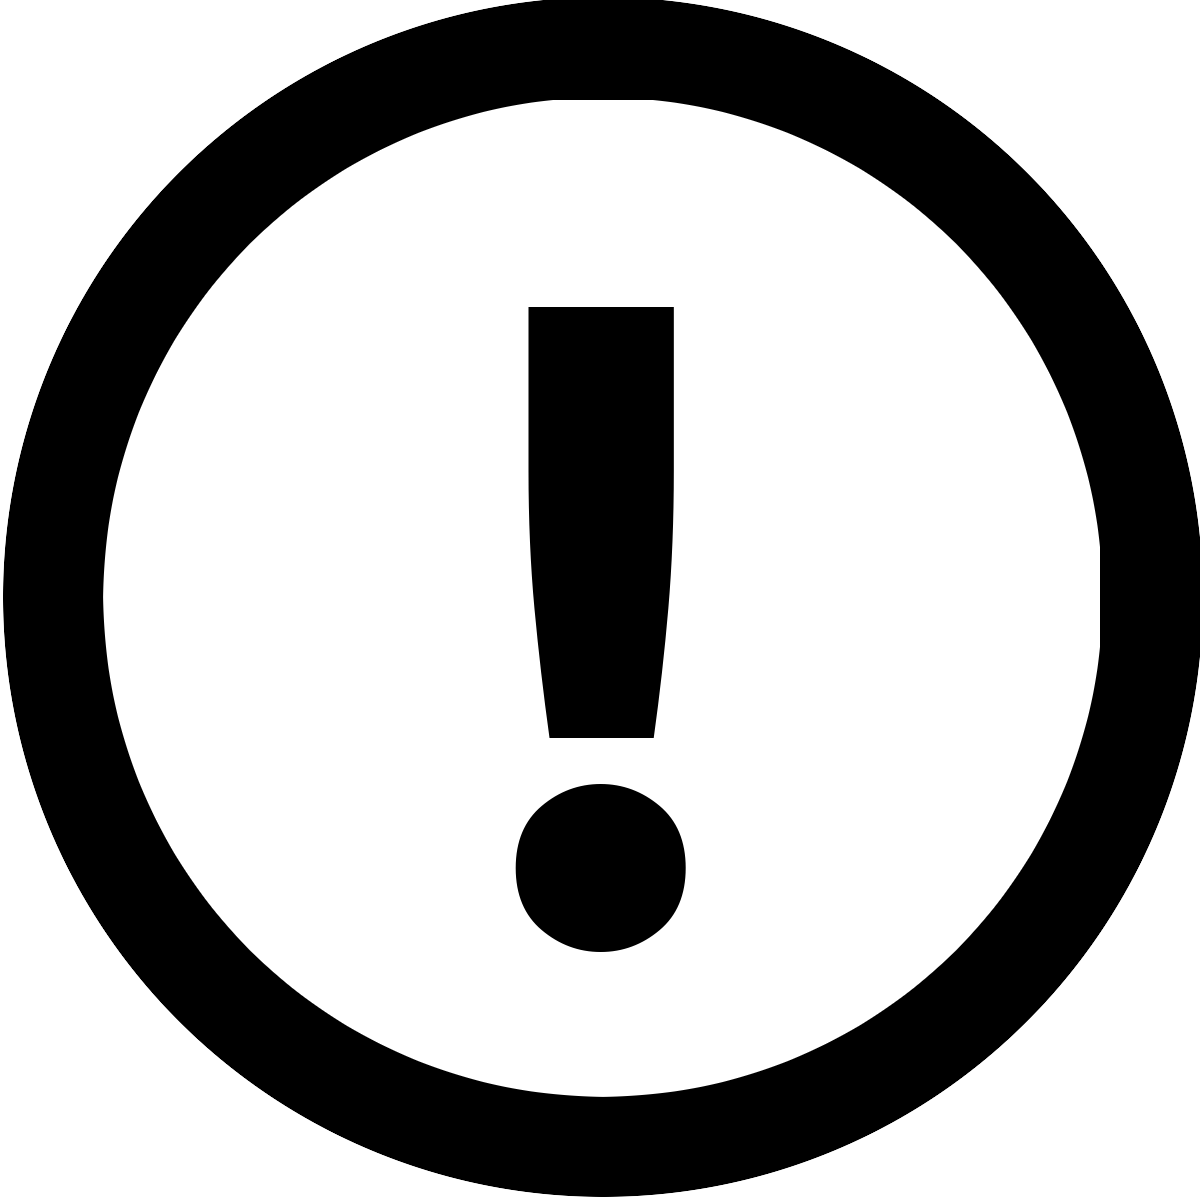
\includegraphics[width=.75\linewidth]{Bilder/recap}
            \textsc{\autoref{#1}}
            \vspace{-25pt}
        \end{wrapfigure}
        #2
        \todo[inline]{Racap!}
    \end{minipage}
}

\newcommand{\recap}[2]{
    \setlength{\fboxsep}{1.5em}
    \colorbox{gray!25}{\parbox{\linewidth-2\fboxsep}{\recappage{#1}{#2}}}
}

% sonstige Präambel
% Workaround f�r lstlistoflistings --------------------------------
\makeatletter
\@ifundefined{float@listhead}{}{%
    \renewcommand*{\lstlistoflistings}{%
        \begingroup
    	    \if@twocolumn
                \@restonecoltrue\onecolumn
            \else
                \@restonecolfalse
            \fi
            \float@listhead{\lstlistlistingname}%
            \setlength{\parskip}{\z@}%
            \setlength{\parindent}{\z@}%
            \setlength{\parfillskip}{\z@ \@plus 1fil}%
            \@starttoc{lol}%
            \if@restonecol\twocolumn\fi
        \endgroup
    }%
}
\makeatother

% Nummerierungstiefe
\setcounter{secnumdepth}{3}
\setcounter{tocdepth}{3}

% Farben
\definecolor{LightGray}{gray}{0.95}

\lstdefinelanguage{QML} 
{morekeywords={color,background,margin, visible, width, height, title, id, fill, text, anchors, centerIn, onClicked, host, onMessageReceived, Component.onCompleted, Component, onCompleted}, 
	emph={ApplicationWindow, Rectangle, Button, QmlQmqtt},
	sensitive=false, 
	morecomment=[l]{//}, 
	morecomment=[s]{/*}{*/},
	morestring=[b]", 
} 


\lstdefinelanguage{json}  
{
	emph={:, \,},
	sensitive=false, 
	morecomment=[l]{//}, 
	morecomment=[s]{/*}{*/},
	morestring=[b]", 
} 

\newcommand{\specialcell}[2][c]{%
	\begin{tabular}[#1]{@{}c@{}}#2\end{tabular}}

% Das eigentliche Dokument -----------------------------------------------------
%   Der eigentliche Inhalt des Dokuments beginnt hier. Die einzelnen Seiten
%   und Kapitel werden in eigene Dateien ausgelagert und hier nur inkludiert.
% ------------------------------------------------------------------------------

\begin{document}
    % Listing Nummern je mit Kapitelnummer
    %\counterwithin{listing}{section}

    % Deckblatt ---------------------------------
    \includepdf[pages=-]{Sonstiges/Deckblatt.pdf}

    % Seitennummerierung: Römische Ziffern; Zurücksetzen auf 1
    \pagenumbering{Roman}
    \setcounter{page}{1}
    
    %\chapter*{Lizenzen}
\addcontentsline{toc}{chapter}{Lizenzen}

\begin{center}

\topskip0pt
\vspace*{\fill}

\quotes{\thema} von \autor\space ist lizenziert unter einer Creative Commons Namensnennung - Nicht-kommerziell - Weitergabe unter gleichen Bedingungen 4.0 International Lizenz (CC BY-NC-SA 4.0). \\

\includegraphics[width=0.2\textwidth]{Bilder/by-nc-sa-eu}\\
\url{http://creativecommons.org/licenses/by-nc-sa/4.0/}

\vspace*{\fill}

Sämtliche in der Arbeit beschriebenen und auf etwaig beigelegten Datenträgern
vorhandenen Ergebnisse dieser Arbeit in Form von Quelltexten, Software und
Konzeptentwürfen sind, sofern nicht anders angegeben, lizenziert unter \quotes{The MIT License (MIT)}. \\

\includegraphics[width=0.1\textwidth]{Bilder/mit_license}\\
\url{https://opensource.org/licenses/MIT}

\vspace*{\fill}

Die LaTeX-Vorlage beruht auf den Inhalten unter\\
\url{http://f.macke.it/MasterarbeitZIP}.

\vspace*{\fill}

{\large \copyright \space 2018 \space \autor}

\vspace*{\fill}

\end{center}
  % Lizenztexte
    
    % Ueberblick --------------------------------
    	\chapter*{Zusammenfassung} \chapter*{Zusammenfassung} \addcontentsline{toc}{chapter}{Zusammenfassung}

Da die \quotes{\textbf{Co}mmon \textbf{B}usiness \textbf{O}riented \textbf{L}anguage}, kurz \mbox{COBOL} genannt, bereits Ende der 1950er Jahre entstand und daher nur wenige moderne Sprachkonzepte bietet, wird der Fokus in der Ausbildung neuer Informatiker immer mehr auf Programmiersprachen mit moderneren objektorientierten Konzepten gelegt. Dem steht gegenüber, dass COBOL immer noch wichtiger Bestandteil bestehender betrieblicher Informationssysteme ist, die es zu warten und zu erweitern gilt. Während diese Sprache heutzutage also zunehmend seltener Teil der Ausbildung von Programmierern ist, besteht, durch die Vielzahl vorhandener COBOL-Systeme, weiterhin eine hohe Nachfrage nach Experten.

Diese Arbeit gibt einen generellen Überblick über Herausforderungen, die sich in Verbindung mit betrieblichen Informationssystemen ergeben, und zeigt, wie COBOL und Java diesen Problemen begegnen. Ferner wird COBOL konzeptuell erfasst und mit Java, als Vertreter moderner Sprachen, verglichen. Dabei steht stets die praktische Anwendung der Sprachen im Vordergrund, weshalb Experteninterviews geführt wurden, um neben bestehender Fachliteratur bestmögliche Einsicht in die Entwicklung und Wartung angesprochener Systeme zu erhalten. Damit entstand ein Leitfaden, der es Programmierern mit Java-Kenntnissen erlaubt, sich mit COBOL vertraut zu machen, indem bekannte Konzepte, Muster und Konstrukte gegenübergestellt werden. Zusätzlich wird, als Ergebnis der Experteninterviews, darauf hingewiesen, wie sich der Umgang mit diesen Konzepten in der Praxis gestaltet und gestalten sollte. 
	\chapter*{Abstract} \chapter*{Abstract} \addcontentsline{toc}{chapter}{Abstract}

COBOL, which stands for the \quotes{\textbf{Co}mmon \textbf{B}usiness \textbf{O}riented \textbf{L}anguage}, began to rise in the late 1950s as a project of the US government. The aim was to design a programming language, which enables persons without knowledge of programming to engineer software systems. At that time nobody could forebode, that it's still used in many existing operational information systems and not uncommon that these have different requirements than modern desktop or web applications regarding the environment and development. So, whilst COBOL is getting less and less attention of new programmers the demand for highly trained and experienced professionals is high yet. This thesis outlines key challenges in terms of those operational information systems and reveals how COBOL copes with them. Furthermore, COBOL gets conceptually surveyed and compared with Java, which represents state of the art programming languages. The practical approach is always on focus in this comparison, and therefore, along with available literature, experts were interviewed to get the best possible insight of development and maintenance of those systems. The purpose was to devise a guide for Java developers, which enables them to familiarize with COBOL by contrasting known concepts, pattern and constructs. The interviews led to best practice advices in combination with those concept descriptions and hints on how those are used in practice and how they should be.
    
%   \singlespacing{
        \tableofcontents                    % Inhaltsverzeichnis
        \listoffigures                      % Abbildungsverzeichnis
        \lstlistoflistings                  % Quellcode-Listings
        \listoftables                       % Tabellenverzeichnis
        \chapter*{\hypertarget{listofnomenclaturelink}{Abkürzungsverzeichnis}}
\addcontentsline{toc}{chapter}{Abkürzungsverzeichnis}


\begin{acronym}[OPC HDA ]
	\acro{AMQP}{Advanced Message Queuing Protocol}
\acro{API}{Programmierschnittstelle}
\acro{APK}{Android application package}
\acro{CEP}{Complex Event Processing}
\acro{COM}{Component Object Model}
\acro{CPS}{Cyber-physisches System}
\acro{DCOM}{Distributed COM}
\acro{DDS}{Data Distribution Service}
\acro{DSG}{Distributed Systems Group}
\acro{GCC}{GNU Compiler Collection}
\acro{GCM}{Google Cloud Messaging}
\acro{GUI}{Graphical User Interface}
\acro{HMI}{Human-Machine-Interface}
\acro{IDE}{Integrated Development Environment}
\acro{IoT}{Internet der Dinge}
\acro{JDK}{Java Development Kit}
\acro{LHS}{left-hand side}
\acro{M2M}{Maschine-zu-Maschine}
\acro{moc}{Meta-Object Compiler}
\acro{MQTT}{Message Queue Telemetry Transport}
\acro{NDK}{Native Development Kit}
\acro{OASIS}{Organization for the Advancement of Structured Information Standards}
\acro{OPC A/E}{OPC Alarms and Events}
\acro{OPC DA}{OPC Data Access}
\acro{OPC DX}{OPC Data exchange}
\acro{OPC HDA}{OPC Historical Data Access}
\acro{OPC UA}{OPC Unified Architecture}
\acro{OPC}{Open Platform Communications}
\acro{PLC}{Programmable Logic Controller}
\acro{QML}{Qt Meta-object Language}
\acro{QoS}{Quality of Service}
\acro{RHS}{right-hand side}
\acro{SCADA}{Supervisory Control and Data Acquisition}
\acro{SDK}{Software Development Kit}
\acro{SPS}{Speicherprogrammierbare Steuerung}
\acro{WSN}{Wireless Sensor Network}
\end{acronym}      % Abkürzungsverzeichnis
%   }
    
    % Zeilenabstand setzen
    \onehalfspacing
    
    % Seitennummerierung: Speichern der Seitennumber in RomanSiteCounter; Arabische Ziffern; Zurücksetzen auf 1
    \pagebreak
    \newcounter{RomanSiteCounter}
    \setcounter{RomanSiteCounter}{\value{page}}
    \pagenumbering{arabic}
    \setcounter{page}{1}
    
    % Inhalt ------------------------------------
        % Einleitung ----------------------------
            \chapter{Einleitung} 



\label{ch:einleitung}
    %\section{Typographische Konventionen}
In diesem Abschnitt werden typographische Konventionen festgelegt, um das Verständnis zu erleichtern.
\begin{itemize}
	
	\item	Fachbegriffe werden \Fachbegriff{kursiv} geschrieben.
	
	\item	Zitate werden in \quotes{doppelten Anführungszeichen} geschrieben.
	
	\item	Quellcode wird in \mintinline{text}{Festschrittschrift} geschrieben.
	\item	Neue und wichtige Begriffe werden \NeuerBegriff{fett} geschrieben.
	
	\item	Abkürzungen werden bei der ersten Verwendung ausgeschrieben und können zusätzlich im
			\hyperlink{listofnomenclaturelink}{Abkürzungsverzeichnis} nachgeschlagen werden.
\end{itemize}
    \section{Problemstellung}\label{problemstellung}
Der folgende Abschnitt soll die Problemstellung verdeutlichen, welche der Arbeit zu Grunde liegt. 
Dazu wird erläutert, welche Wichtigkeit COBOL genießt und anschließend mit der Bedeutung, die der Sprache in der Lehre tatsächlich beigemessen wird und den Folgen davon für den Arbeitsmarkt, gegenübergestellt.

\subsection*{Wichtigkeit von COBOL}\label{wichtigkeit}
\quotes{Viele Millionen Cobol-Programme existieren weltweit und müssen laufend gepflegt werden.
Es ist bei dieser Situation undenkbar und unter wirtschaftlichen Gesichtspunkten unvertretbar in den nächsten Jahren eine Umstellung dieser Programme auf eine andere Sprache durchzuführen.} \cite{_ist_1979}

Was Herr Dr. Strunz neben vielen anderen Experten bereits 1979 prophezeite hat auch heute noch Gültigkeit. Obwohl COBOL zum Ende der 50er Jahre entstand, 1959 veröffentlicht wurde und damit fast 60 Jahre alt ist, trifft man es auch heute noch häufig an. In der britischen Tageszeitung The Guardian, zitiert der Autor Scott Colvey in seinem Artikel %``\citefield{colvey_cobol_2009}{title}'' 
\cite{colvey_cobol_2009} anlässlich des 50. Geburtstages von COBOL den Micro Focus Manager David Stephenson: \quotes{`some 70\% to 80\% of UK plc business transactions are still based on Cobol'}. 
Weiter führt er darin Aussagen von IBM Software-Leiters Charles Chu an, welcher die Aussagen von Stephenson bestätigt: \quotes{$[\ldots]$ there are 250bn lines of Cobol code working well worldwide. Why would companies replace systems that are working well?'}. 
Stephen Kelly, Geschäftsführer von Micro Focus, betont zudem, dass sich Stand 2009 über 220 Milliarden COBOL-Codezeilen im produktiven Einsatz befanden, welche vermutlich 80\% der insgesamt weltweit aktiven Codezeilen ausmachten. Außerdem wurden damaligen Zeitpunkt wurden geschätzt 200-mal mehr COBOL-Transaktionen ausgeführt als Google Suchanfragen verzeichnen konnte. \cite{kelly_cobol_2009} Diese Aussagen decken sich mit den Angaben in \citeWithTitle{doke_cobol_2005}. Auch darin heißt es, dass mit 225 Milliarden Codezeilen, etwa 70\% des weltweiten Codes in COBOL geschrieben sind.

Nicht nur, dass COBOL in den vergangenen Jahren also einen enormen Marktanteil ausmachte wird also deutlich, sondern auch die Bedeutung für die Zukunft: Wieso sollte funktionierender Code mit Hilfe von teuren und riskanten Prozessen ersetzt werden?

Da sich viele Unternehmen der Frage eines Umstiegs von COBOL auf eine modernere Lösung ausgesetzt sehen, auf die sich nur schwer eine Antwort finden lässt, welche die Risiken und Kosten aufwiegt, stieg die Anzahl \todo[inline]{Beleg} des sich weltweit in Produktion befindlichen COBOL-Codes über die vergangen Jahre sogar noch weiter an.
Dieses Risiko ergibt sich vorrangig durch die Trasnaktion immenser Geldsummen, die mit COBOL-Systemen durchgeführt werden: \quotes{Täglich werden Transaktionen mit einem Volumen von schätzungsweise drei Billionen Dollar über Cobol-Systeme abgewickelt. Dabei geht es um Girokonten, Kartennetze, Geldautomaten und die Abwicklung von Immobilienkrediten. Weil die Banken aggressiv auf eine Digitalisierung ihres Geschäftes setzen, wird Cobol sogar noch wichtiger. Denn Apps für Smartphones etwa sind in modernen Sprachen geschrieben, müssen aber mit den alten Systemen harmonieren.} \cite{beat_balzli_cobol-programmierer_2017}

Im TIOBE-Index\cite{_tiobe_} für April 2018 rangiert COBOL auf Platz 25 mit einem Rating von 0.541\%. Dieser Index wird auf Basis von Suchanfragen nach den entsprechenden Programmiersprachen, auf den meist frequentiertesten Internetseiten, erstellt. COBOL ist somit zwar nur Teil jeder 200. Suchanfrage, rangiert jedoch damit trotzdem vor anderen etablierten oder aufstrebenden Sprachen wie \textit{Kotlin}, \textit{Scala} oder \textit{Haskell}. Außerdem gilt es hier zu beachten, dass COBOL zu einer Zeit entstand, in der das Internet noch lange nicht existierte und Informationen über die Sprache mittels Büchern verbreitet und vermittelt wurden. Daher ist auch heute noch das Internet nicht die vorrangige Quelle, um Wissen über COBOL zu akquirieren. Unter diesen Gesichtspunkten ist das TIOBE-Rating von COBOL als noch höher einzuschätzen.


\subsection*{Bedeutung in der Lehre}
Da COBOL bereits 60 Jahre alt ist haben heutzutage bereits viele einstige COBOL-Entwickler das Rentenalter erreicht. Im Artikel \citeWithTitle{beat_balzli_cobol-programmierer_2017} beschreibt der Autor exemplarisch den Fall eines 75-jährigen Entwickler, der ob seiner Erfahrung und trotz seines Alters immernoch in der Branche tätig ist.

Junge COBOL-Entwickler sind rar, da COBOL nur noch selten Teil der Ausbildung ist. \citeauthor{doke_cobol_2005} führen in \citeWithTitle{doke_cobol_2005} an, dass im Jahr 2002 lediglich in 36.2\% COBOL Teil des Gundstudiums war, obwohl im Jahr 1995 noch 89.7\% der befragten Bildungseinrichtungen angaben COBOL-Kurse als festen Bestandteil der Ausbildung zu haben. Sieht man sich dagegen die Zahlen zu Java als Vertreter moderner Programmiersprachen an, lässt sich ein klarer Trend erkennen. Erst 1995 entstanden, stieg die Zahl der  Universitäten, die Java lehrten von 42.5\% im Jahr 1998 auf 90.0\% im Jahr 2002. Spinnt man diesen Wandel ins heutige Jahr weiter, zu dem sich in der Zwischenzeit noch eine Fülle neuerer lässt sich erahnen wie selten Lehrveranstaltung zum Thema COBOL inzwischen geworden sind.

Man sieht also, dass sich die Lehrer, obwohl der Bedarf an COBOL-Programmierern weiterhin immens ist, stark weg von COBOL fokussiert hat was die Wirtschaft zusammen mit dem zunehmenden Alter erfahrener COBOL-Entwickler vor Probleme stellt.

\subsection*{Kontroverse Beurteilungen von COBOL}
Die in \autoref{wichtigkeit} angeführten Aussagen und Meinungen stammen oftmals von Personen aus dem Umfeld von Unternehmen, die teils hohen Profit aus dem Weiterbestehen COBOLs herausschlagen. Diese Aussagen sind daher, wenn auch sicherlich nicht falsch, vorsichtig und vor allem sehr differenziert zu betrachten.

Der mehrfach prämierte Informatiker \citeauthor{edsger_wybe_dijkstra_how_1975} z.B. findet sehr klare andere Worte zu COBOL: \quotes{The use of COBOL cripples the mind; its teaching should, therefore, be regarded as a criminal offence.} \cite{edsger_wybe_dijkstra_how_1975}

\citeauthor{florian_hamann_banken_2017} nennt in seinem Artikel \citeWithTitle{florian_hamann_banken_2017} die bereits erwähnte zunehmende Knappheit von Arbeitskräften auch als einen wichtigen Faktor dafür, weshalb COBOL über kurz oder lang von moderneren Systemen und Sprachen verdrängt und abgelöst wird.

Trotz dieser Kontroversen kann festgehalten werden, dass es nach wie vor eine gleichbleibend hohen Bedarf an Entwicklern gibt, den es zu decken gilt.
    \section{Ziel der Arbeit}
Die vorliegende Arbeit leistet einen Beitrag zur Lösung der in \autoref{problemstellung} beschriebenen Probleme. Dies geschieht mithilfe eines Leitfadens, der fachkundigen Java-Entwicklern den Einstieg in COBOL erleichtert, indem gängige Sprachkonzepte gegenübergestellt und verglichen werden. 

Das ermöglicht es, vorhandenes Wissen über Softwareentwicklung, im speziellen mit Java, in einen COBOL-Kontext zu bringen und passende Sprachkonzepte nutzen zu lernen. Des Weiteren wird aufgezeigt, welche konzeptuellen Herausforderungen sich bei der COBOL-Entwicklung und Migration ergeben.

Im Fokus steht hierbei neben der Einführung in relevante Sprachkonstrukte stets auch die Experteneinschätzung zur Nutzung der verschiedenen Konzepte. Daher wird, wenn möglich, zusätzlich zu den erklärten Paradigmen erläutert, wie die Verwendung in der Praxis aussehen \bzw nicht aussehen sollte und je nach Sprachmittel gegebenenfalls in der Praxis zu verwendende Alternativen aufgezeigt.

Es ist nicht Ziel der Arbeit, vorhandene Java-Entwickler zu Neuentwicklungen mit COBOL zu animieren oder diese gar zu COBOL-Entwicklern umzuschulen. Wichtig ist in diesem Zusammenhang vielmehr, ihr Wissensspektrum so zu erweitern, dass es ihnen möglich wird, komplexe fachliche Zusammenhänge, vor allem die \quotes{business logic}, bestehender COBOL-Architekturen zu erkennen und zu verstehen. Dadurch sind diese Entwickler flexibler einsetzbar und geschult, um mit Migrations-, Renovierungs- und Wartungsaufgaben von COBOL-Systemen betraut werden zu können.

Neben den praxisrelevanten Aspekten erfasst diese Arbeit Java und COBOL konzeptuell und bringt die Sprachen so in einen universitären Kontext. Dies dient dem Zweck, die zugrunde liegenden Ansätze statt deren syntaktischer Schreibweisen zu untersuchen. Außerdem werden dabei bekannte, in der Praxis häufig zu findende Muster beleuchtet und mit den zutage geförderten Kernkonzepten der Sprachen verglichen, um Aufschluss darüber zu geben, wie die Sprachkonzepte in der Praxis angewendet \bzw genutzt werden.
	\section{Aufbau der Arbeit}
        % Stand der Technik ---------------------
        %    \input{StandDerTechnik/StandDerTechnik}
        % Wissenschaftliche Lücke ---------------
        %    \input{AufgabenstellungUndAnforderung/AufgabenstellungUndAnforderung}
        % Umsetzung -----------------------------
        %    \input{Umsetzung/Umsetzung}
        % Ergebnisse und Evaluation -------------
        %    \input{ErgebnisseUndEvaluation/ErgebnisseUndEvaluation}
        % Schluss -------------------------------
        %    \section{Fazit}
    
    % Seitennummerierung: Römische Ziffern; Zurücksetzen auf in RomanSiteCounter gespeicherten Wert.
    \pagebreak
    \pagenumbering{Roman}
    \setcounter{page}{\value{RomanSiteCounter}}
    
    % Literatur ---------------------------------
    \nocite{*}
    \ohead{\textit{Literaturverzeichnis}}
    \singlespacing
    \bibliography{Sonstiges/Bibliothek}
    \pagebreak
    
    % Eidesstattliche Erklärung -----------------
    %\pagebreak
\ohead{\textit{Eidesstattliche Erkl�rung}}
\chapter*{Eidesstattliche Erkl�rung} 
\addcontentsline{toc}{chapter}{Eidesstattliche Erkl�rung}

Hiermit erkl�re ich, \autor, Matrikel-Nr. \matrikelnr, an Eides statt, dass ich die vorliegende Arbeit mit dem Thema

\begin{center}
\textbf{\quotes{\titel}} 
\end{center}

selbstst�ndig und unter Verwendung der angegebenen Quellen und Hilfsmittel erstellt
habe. Ich habe die vorliegende Arbeit nicht anderweitig f�r Pr�fungszwecke
vorgelegt.

\bigskip\bigskip\bigskip\bigskip\bigskip\bigskip


\ort, \today

\hspace*{\fill}\begin{tabular}{@{}l@{}}\hline
\makebox[6cm]{\autor}
\end{tabular}
\pagebreak
    
    % Anhänge -----------------------------------
    \ohead{\textit{Anhang}}
    %\appendix
\chapter{Inhalt des beigefügten Datenträgers}\label{chap:appendix_dvd}
% \begin{itemize}
%   \item \textbf{./Application/Android} 
%   Android APKs des Frontends
%   \item \textbf{./Application/Linux\_x64} 
%   Linux Bibliotheken und ausführbare Datei (64-Bit)
%   \item \textbf{./Application/Linux\_x86} 
%   Linux Bibliotheken und ausführbare Datei (32-Bit)
%   \item \textbf{./Application/Windows/Alarming\_App.zip} 
%   Windows Bibliotheken und ausführbare Datei (32-Bit; gepackt)
%   \item \textbf{./Code/Backend/module\_opc} 
%   Kommentierter Quellcode des OPC-Moduls  
%   \item \textbf{./Code/Backend/module\_rules} 
%   Kommentierter Quellcode des Regelmoduls
%   \item \textbf{./Code/Frontend/Alarming\_App} 
%   Kommentierter Quellcode der Alarming-App
%   \item \textbf{./Code/Frontend/Alarming\_Service} 
%   Kommentierter Quellcode des Alarming-Service
%   \item \textbf{./Diagrams} 
%   Diagramme zum entwickelten Code
%   \item \textbf{./Doc} 
%   Quelltext-Dokumentationen
%   \item \textbf{./Thesis/Bachelorarbeit\_Antonio\_Grieco\_930190.pdf} 
%   PDF dieser Arbeit
%   \item \textbf{./Thesis/Latex} 
%   Arbeit im Latex-Format
%   \item \textbf{./VM} 
%   Virtuelle Maschine mit lauffähiger Umgebung
%   \item \textbf{./Zotero-Bibliothek} 
%   Komplette Zotero-Bibliothek zur Arbeit mit Snapshots und Dokumenten
% \end{itemize}
    
\end{document}
